\section{Technology}
\label{sec:Technology}
The design of this active balun is implemented in the SG13G3 technology, developed by IHP-Innovations for High Performance Microelectronics.
SG13G3 \cite{SiG13G3} is the evolution of the SiGe BiCMOS G2 technology and offers a peak $f_T$ of \SI{500}{\giga\hertz} and a peak $f_{\mathrm{MAX}}$ of \SI{610}{\giga\hertz}.

\begin{figure}[hbt!]
    \centering
       \begin{circuitikz}[scale=0.95,transform shape]
        
        % Transistor
        \draw (0,0) node[npn, anchor=B] (Q1)
        {\shortstack{$Q$}};
        
        % Base branch
        \draw (Q1.B) to [short]++(-0.25,0) coordinate (vb1);
        \draw (vb1) --++(-0.25,0) coordinate(b1)
              to [C]++(-2,0) 
              to [short]++(-0.25,0) coordinate(in);
        \draw (vb1) coordinate(e1)
              to [L,*-]++(0,-2.25) to [vsource,l=$\mathrm{V}_{\mathrm{B}}$]++(0,-1) node[ground]{};
        
        % Collector branch
        \draw (Q1.C) to [short,-*]++ (0,0.25) coordinate(c1) 
        --++ (0,0.1) to [L,mirror]++(0,2)
              to [open]++(-0.35,0) -- node[anchor=south] {$\mathrm{V}_{\mathrm{CC}}$} ++(0.7,0);
        \draw (c1) --++(0.25,0) to [C]++(2,0) to [short]++(0.25,0)coordinate(out);
        
        % Emitter branch
        \draw (Q1.E) --++(0,0) node[ground]{};
        
        % Highlight rectangles
        \draw (c1) to [open]++(-0.35,0.4) rectangle++(0.75,1.25);
        \draw (c1) to [open]++(0.25+0.5,-0.425) rectangle++(1.0,0.85);
        \draw (e1) to [open]++(-0.35,-0.5) rectangle++(0.75,-1.25);
        \draw (b1) to [open]++(-0.5,-0.425) rectangle++(-1.0,0.85);

        %% TermG in
        \def\Sc{0.8}
        \begin{scope}[scale=\Sc,transform shape]
        \draw (in) 
            to [short] ++(0, -0.5) 
            to [R] ++(0, -1.85) node[tlground] {};
        \draw (in) ++(-0.5,-0.65) rectangle ++(1, -2.05);
        % label
       % \draw (in)++(-1,-1.775) node[]{\Huge{$Z_0$}};
    \end{scope}
    % termG out
    \begin{scope}[scale=\Sc,transform shape]
        \draw (out) 
            to [short] ++(0, -0.5) 
            to [R] ++(0, -1.85) node[tlground] {};
        \draw (out) ++(+0.5,-0.65) rectangle ++(-1, -2.05);
        % label
       % \draw (in)++(-1,-1.775) node[]{\Huge{$Z_0$}};
    \end{scope}
        \end{circuitikz}

    \caption{Schematic simulation of the SG13G3}
    \label{fig:FtFmaxSchematic}
\end{figure}

 \begin{figure}[hbt!]
     \centering
     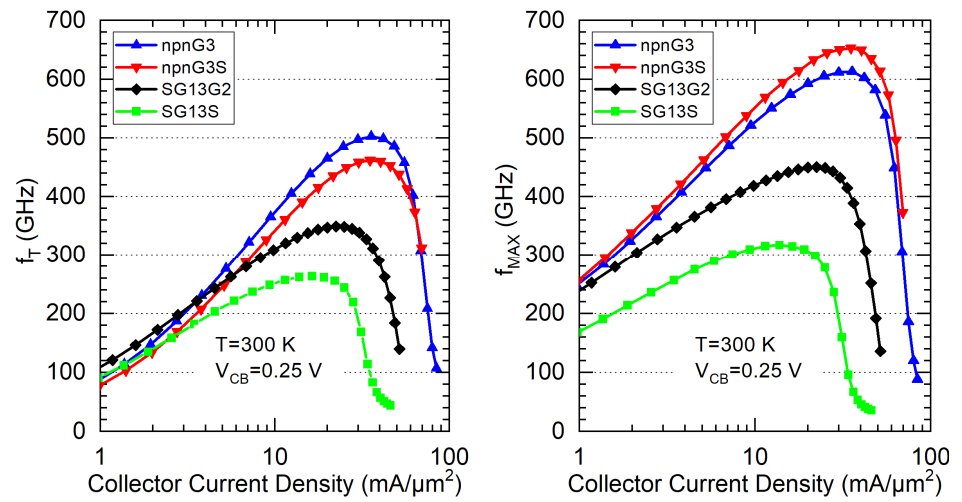
\includegraphics[width=0.85\linewidth]{Design_figures/FtFmaxSG13G3.png}
    \caption{$f_T$ and $f_{\mathrm{MAX}}$ of the high-speed HBTs npnG3 ($A_E=0.1\times0.97\,\mu\mathrm{m}^2$) and npnG3S ($A_E=0.1\times0.45\,\mu\mathrm{m}^2$) as a function of the collector current density. Figure taken from \cite{SiG13G3}.}
     \label{fig:FtFmaxSG13G3}
 \end{figure}

 \cleardoublepage
\subsection{Layer stack}
The technology description can be found in the open-source SG13G2 PDK \cite{SiG13G2} as well as in the paper \cite{SiG13G3}.\
SG13G3 is a high-performance BiCMOS technology based on a \SI{0.13}{\micro\meter} CMOS process. It includes bipolar devices based on SiGe:C npn-HBTs, as well as passive components such as polysilicon resistors and MIM capacitors.

\begin{figure}[hbt!]
    \centering
    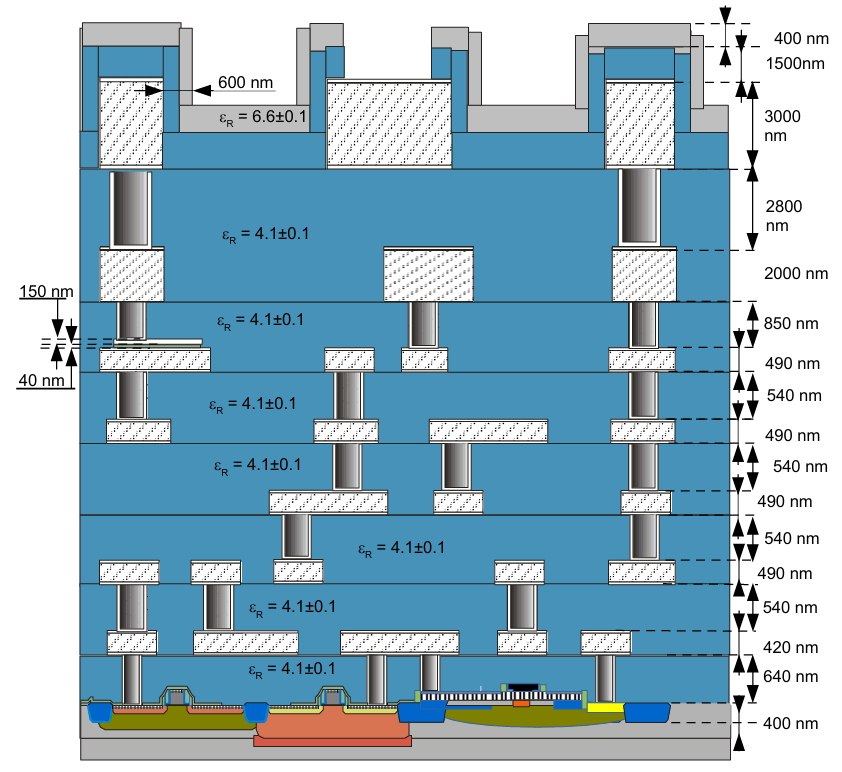
\includegraphics[width=0.75\linewidth]{CrossSectionSchematicSG13G2.png}
    \caption{Cross section of the SG13G3 process from the Open PDK GitHub\cite{SiG13G2}.}
    \label{fig:CrossSectionSchematicSG13G2}
\end{figure}

The SG13G2 technology layer cross section is shown in Figure~\ref{fig:CrossSectionSchematicSG13G2}.\\
MOM capacitors are realized using TopMetal1 and Metal5, while the transmission lines are mostly realized in TopMetal2.

The technology has a total of seven layers, excluding the active layer. The back end offers five thin metal layers, two thick metal layers (\SI{2}{\micro\meter} and \SI{3}{\micro\meter} thick) to support high current and low losses, and a MIM layer. The transistors are realized in the active layer, and their terminals are made available through metal vias. In particular, the base and collector are connected to Metal1, while the emitter is connected to Metal2.

In this design, Metal3 is used as the source plane, while Metal4 is used as the ground plane.

\begin{comment}
The RF signals enters from the the external layer, TopMetal2.

Metal1 (M1) – il layer più basso, usato soprattutto per routing locale vicino ai transistor.

Metal2 (M2) → Metal3 (M3) → Metal4 (M4) → Metal5 (M5) – routing progressivo, con M3/M4 spesso usati per reti globali e plane GND/VDD, e gli altri principalmente per segnali o routing di blocco.

TopMetal1 / TopMetal2 – strati spessi, larghe piste per alimentazione, massa, o segnali RF ad alta corrente, e piste di trasmissione a bassa perdita.


The sensible components are shielded from the RF signal by the RF ground in Metal4. 
The Voltage supply is in metal 3
\end{comment}